\documentclass[12pt]{article}

\usepackage[utf8]{inputenc}
\usepackage{latexsym,amsfonts,amssymb,amsthm,amsmath}
\usepackage{tikz}
\usepackage{stanli}
\usetikzlibrary{shapes,calc,through,3d,patterns}
\usetikzlibrary{arrows.meta,decorations.pathreplacing,angles,quotes}
\usepackage{multicol}
\usepackage{geometry}
\usepackage{mathtools}
\usepackage{siunitx}
\usepackage{booktabs}

\setlength{\parindent}{0in}
\setlength{\oddsidemargin}{-0.25in}
\setlength{\textwidth}{7in}
\setlength{\textheight}{9.3in}
\setlength{\topmargin}{-1in}
\setlength{\headheight}{18pt}

\newcommand\blfootnote[1]{%
    \begingroup
    \renewcommand\thefootnote{}\footnote{#1}%
    \addtocounter{footnote}{-1}%
    \endgroup
}

\definecolor{darkred}{rgb}{0.6,0,0}

\newcommand{\bolddelta}{\boldsymbol\delta}
\newcommand{\boldxi}{\boldsymbol\xi}

\begin{document}

\noindent ME473 - Dynamic finite element analysis of structures\hfill EPFL\\
Stefano Burzio \hfill 2025\\
\vspace{0.3cm}

\hspace*{\fill}\textbf{\Large Problem set 8}\hspace*{\fill}

\hrulefill

\subsection*{Problem 1}
Consider the free vibration analysis of a square Reissner-Mindlin plate discretized using a structured mesh of $2 \times 2$ bilinear quadrilateral finite elements, as illustrated in the figure below. The domain is divided into four bilinear elements.
\begin{center}
  \begin{tikzpicture}[scale=1]
    \def\a{4}
    \def\b{4}
    % Draw the rectangle
    \filldraw[fill=gray!60, draw=black,thick] (0,0) rectangle (\a,\b);
    % Draw the elements  
    \draw[thick] (\a/2,0) -- (\a/2,\b);
    \draw[thick] (0,\b/2) -- (\a,\b/2);
    \node at (\a/4,\b/4) {${}^1\Omega$};
    \node at (\a/4,3*\b/4) {${}^2\Omega$};
    \node at (3*\a/4,\b/4) {${}^3\Omega$};
    \node at (3*\a/4,3*\b/4) {${}^4\Omega$};
    %axis
    \draw[-latex,ultra thin] (-0.5,0) -- (\a+1,0) node[right]{$x$};
    \draw[-latex, ultra thin] (0,-0.5) -- (0,\b+1)node[above]{$y$};
    % length
    \draw[latex-latex, ultra thin]  (0,\b+0.5)  to node[midway,above] {$a$}(\a/2,\b+0.5) ;
    \draw[latex-latex, ultra thin]  (\a/2,\b+0.5)  to node[midway,above] {$a$}(\a,\b+0.5) ;
    \draw[ultra thin] (\a/2,0) --(\a/2, \b+1);
    \draw[ultra thin] (\a,0) --(\a, \b+1) ;
    \draw[ultra thin] (0,\b/2) --(\a+1, \b/2);
    \draw[ultra thin] (0,\b) --(\a+1, \b);
    \draw[ultra thin] (\a,0) -- (\a+1,0);
    \draw[ultra thin] (0,\b) -- (0,\b+1);
    \draw[latex-latex, ultra thin]  (\a+0.8,\b/2)  to node[midway,right] {$a$}(\a+0.8,0) ;
    \draw[latex-latex, ultra thin]  (\a+0.8,\b)  to node[midway,right] {$a$}(\a+0.8,\b/2) ;
    % Nodes 
    \draw[fill=white, draw=black]  (0,0) node[below right]{$\mathbf x_1$} circle (3pt);
    \draw[fill=white, draw=black]  (0,\b/2) node[below right]{$\mathbf x_2$} circle (3pt);
    \draw[fill=white, draw=black]  (0,\b) node[below right]{$\mathbf x_3$} circle (3pt);
    \draw[fill=white, draw=black]  (\a/2,0) node[below right]{$\mathbf x_4$} circle (3pt);
    \draw[fill=white, draw=black]  (\a/2,\b/2) node[below right]{$\mathbf x_5$} circle (3pt);
    \draw[fill=white, draw=black]  (\a/2,\b) node[below right]{$\mathbf x_6$} circle (3pt);
    \draw[fill=white, draw=black]  (\a,0) node[below right]{$\mathbf x_7$} circle (3pt);
    \draw[fill=white, draw=black]  (\a,\b/2) node[below right]{$\mathbf x_8$} circle (3pt);
    \draw[fill=white, draw=black]  (\a,\b) node[below right]{$\mathbf x_9$} circle (3pt);
  \end{tikzpicture}
\end{center}
For each of the following boundary conditions, determine which degrees of freedom in the system are free:
\begin{enumerate}
  \item Clamped on all four edges. This boundary condition is often referred
        to by the acronym CCCC.
  \item Two edges parallels to the $x$-axis are simply supported and two edges parallels to the $y$-axis are free. This boundary condition is often referred to by the acronym SFSF.
  \item Corner nodes are simply supported only. This boundary condition is often referred to by: corners-SSSS.
\end{enumerate}
For which boundary conditions do you expect the lowest first fundamental frequency?

\subsection*{Problem 2}
Consider a moderately thick square isotropic plate of dimensions $2 \times 2 \times h$ (length $\times$ width $\times$ thickness), as shown in the figure below. The plate is clamped at three of its corners—specifically at nodes $\mathbf{x}_2$, $\mathbf{x}_3$, and $\mathbf{x}_4$—while the fourth corner at $\mathbf{x}_1$ remains free. This boundary condition is often referred to by the acronym FCCC. Discretize the plate using a single bilinear thick-plate finite element. Proceed to compute the reduced stiffness and mass matrices associated with this boundary condition.
\begin{center}
  \begin{tikzpicture}[scale=0.7]
    \def\a{4}
    \def\b{4}
    % Draw the rectangle
    \filldraw[fill=gray!60, draw=black,thick] (0,0) rectangle (\a,\b);
    % Draw the elements  
    \draw[thick] (\a/2,0) -- (\a/2,\b);
    \draw[thick] (0,\b/2) -- (\a,\b/2);
    %axis
    \draw[-latex,ultra thin] (-0.5,\b/2) -- (\a+1,\b/2) node[right]{$x$};
    \draw[-latex, ultra thin] (\a/2,-0.5) -- (\a/2,\b+1)node[above]{$y$};
    % length
    \draw[latex-latex, ultra thin]  (0,\b+0.5)  to node[midway,above] {$1$}(\a/2,\b+0.5) ;
    \draw[latex-latex, ultra thin]  (\a/2,\b+0.5)  to node[midway,above] {$1$}(\a,\b+0.5) ;
    \draw[ultra thin] (\a/2,0) --(\a/2, \b+1);
    \draw[ultra thin] (\a,0) --(\a, \b+1) ;
    \draw[ultra thin] (0,\b/2) --(\a+1, \b/2);
    \draw[ultra thin] (0,\b) --(\a+1, \b);
    \draw[ultra thin] (\a,0) -- (\a+1,0);
    \draw[ultra thin] (0,\b) -- (0,\b+1);
    \draw[latex-latex, ultra thin]  (\a+0.8,\b/2)  to node[midway,right] {$1$}(\a+0.8,0) ;
    \draw[latex-latex, ultra thin]  (\a+0.8,\b)  to node[midway,right] {$1$}(\a+0.8,\b/2) ;
    % Nodes 
    \draw[fill=white, draw=black]  (0,0) node[below left]{$\mathbf x_1$} circle (3pt);
    \draw[fill=white, draw=black]  (0,\b) node[above left]{$\mathbf x_4$} circle (3pt);
    \draw[fill=white, draw=black]  (\a,0) node[below right]{$\mathbf x_2$} circle (3pt);
    \draw[fill=white, draw=black]  (\a,\b) node[above right]{$\mathbf x_3$} circle (3pt);
  \end{tikzpicture}
\end{center}
The following expressions may be useful in the calculation of the matrices:
\vspace{-0.5cm}
\begin{multicols}{2}
  $$\int_{-1}^1\int_{-1}^1 {}^a h_1^2 \, d\xi_2d\xi_1=\frac{4}{9}$$

  $$\int_{-1}^1\int_{-1}^1 (\partial_{\xi_2}{}^a h_1)^2 \, d\xi_2d\xi_1=\frac{1}{3}$$

  $$\int_{-1}^1\int_{-1}^1  (\partial_{\xi_1}{}^ah_1)^2 \, d\xi_2d\xi_1=\frac{1}{3}$$

  $$\int_{-1}^1\int_{-1}^1  (\partial_{\xi_1}{}^ah_1)(\partial_{\xi_2}{}^ah_1) \, d\xi_2d\xi_1=\frac{1}{4}$$

  $$\int_{-1}^1\int_{-1}^1 ({}^ah_1)(\partial_{\xi_1}{}^ah_1) \, d\xi_2d\xi_1=-\frac{1}{3}$$

  $$\int_{-1}^1\int_{-1}^1 ({}^ah_1)(\partial_{\xi_2}{}^ah_1) \, d\xi_2d\xi_1=-\frac{1}{3}$$
\end{multicols}
The materials parameters of the plate are: $E$ Young's modulus, $\nu$ Poisson ratio and $\rho$ mass density. Moreover the shear correction factor is $k$.


\subsection*{Problem 3}
Analyze the effect of the span-to-thickness ratio on the accuracy of the fundamental frequency of a simply supported isotropic square plate using the finite element method. Modify the provided \texttt{MATLAB} code to evaluate plates with dimensions $1 \times 1 \times h$, where the thickness $h$ takes the following values:
{\small
\begin{table}[h!]
  \centering
  \begin{tabular}{l|c|c}
    \hline
    $h$     & Span-to-thickness ratio & Description            \\
    \hline
    $0.01$  & 100                     & Thin plate             \\
    $0.02$  & 50                      &                        \\
    $0.05$  & 20                      &                        \\
    $0.075$ & 13.333                  &                        \\
    $0.100$ & 10                      & Moderately thick plate \\
    $0.125$ & 8                       &                        \\
    $0.150$ & 6.666                   &                        \\
    $0.5$   & 2                       & Thick plate            \\
    $1$     & 1                       & 3d solid plate         \\
    \hline
  \end{tabular}
\end{table}
}

Discretize each plate using an $8 \times 8$ mesh of bilinear finite elements. For each thickness value, compute the approximated fundamental natural frequency and compare it with the corresponding analytical (exact) value. Discuss the accuracy of the numerical approximation as a function of the span-to-thickness ratio.

To facilitate the implementation, you may employ the provided functions: \texttt{createRectangularMesh}, \texttt{getConstrainedDOFs\_SSSS}, \texttt{formStiffnessThickPlate}, \texttt{formMassThickPlate} and \\ \texttt{computeExactFrequency}.
\end{document}